Da der Punkt dieses Versuches die Fehlerrechnung selbst ist, beinhaltet dieses
Kapitel  ausnahmsweise  auch  die  Fehlerrechnung. \"Ublicherweise  ist  diese
jedoch in einem separaten Kapitel zu finden.

% **************************************************************************** %
\subsection{Aufgabe 1: Schallgeschwindigkeit}
% **************************************************************************** %

\subsubsection{Daten}

\begin{itemize}
    \item
        \emph{L\"ange der Messtrecke}: $\SI[separate-uncertainty = true]{2.561 \pm 0.003 }{\meter}$
    \item
        \emph{Raumtemperatur}: $\vartheta = \SI{23}{\celsius}$
\end{itemize}

Messprotokoll:

\begin{center}
\begin{tabular}{rr|rr}
    \toprule
    Messung & Laufzeit $t_i$ (ms) & Messung & Laufzeit $t_i$ (ms) \\
    \midrule
     1       & 6.83  & 11       & 7.36 \\
     2       & 7.41  & 12       & 7.31 \\
     3       & 7.32  & 13       & 7.56 \\
     4       & 7.31  & 14       & 7.14 \\
     5       & 7.23  & 15       & 6.94 \\
     6       & 7.68  & 16       & 7.32 \\
     7       & 7.33  & 17       & 7.34 \\
     8       & 7.7   & 18       & 7.28 \\
     9       & 7.93  & 19       & 7.01 \\
    10       & 7.54  & 20       & 7.76 \\
    \bottomrule
\end{tabular}
\end{center}


\subsubsection{Mittlere Laufzeit und ihre Unsicherheit}

Mittlere Laufzeit:
\begin{equation}
    \overline{t} = \frac{1}{20} \sum_{i=1}^{20} t_i = \SI{7.37}{\milli\second}
\end{equation}
Fehler des Mittelwertes:
\begin{equation}
    %s_{\overline{t}} = \frac{1}{20} \sum_{i=1}^{20} t_i = \SI{0.01}{\milli\second}
    s_{\overline{t}} = \sqrt{ \frac{\sum_{1}^{20}{(t_i-\overline{t})^2}}{20 \cdot 19}} = \SI{0.062}{\milli\second} \\
\end{equation}

Standardabweichung:
\begin{equation}
    s_{\overline{t}} = \sqrt{ \frac{\sum_{1}^{20}{(t_i-\overline{t})^2}}{19}} = \SI{0.28}{\milli\second} \\
\end{equation}


\subsubsection{Wert und Unsicherheit der Schallgeschwindigkeit}

Es   sind   hier  zwei   Vergleichswerte   aufgef\"uhrt. Der   eine  ist   ein
Tabellenwert    aus   Horst    Kuchling's   \emph{Taschenbuch    der   Physik}
\cite{ref:kuchling:speedOfSoundTable}.    Der  andere   Wert  errechnet   sich
aus   einer    Formel   f\"ur    die   Schallgeschwindigkeit    in   trockener
Luft,   abh\"angig   von  der   Temperatur.  Die   Formel   kann  sowohl   auf
Wikipedia  \cite{ref:wikipedia:speedOfSound}  wie   auch  in  Kuchling's  Werk
\cite{ref:kuchling:speedOfSoundFormula} gefunden werden.

\begin{equation}
    \label{eq:schallgeschwTemperatur}
    c_{luft} = (331.3 + 0.606 \cdot \vartheta) \si{\meter\per\second} = (331.3 + 0.606 \cdot 23) \si{\meter\per\second} = \SI{345.24}{\meter\per\second}
\end{equation}

Der Tabellenwert  aus Kuchling's Buch ist  $\SI{344}{\meter\per\second}$, also
ziemlich nahe beim errechneten Wert.


Berechnung der mittleren Geschwindigkeit:

\begin{gather}
    c = \frac{s}{t} \\
    \overline{c} = \frac{s}{\overline{t}} = \frac{\SI{2.561}{\meter}}{\SI{7.37}{\milli\second}} = \SI{347.73}{\meter\per\second} \\
\end{gather}

Gauss'sches Fehlerfortpflanzungsgesetz:
\begin{equation}
    s_{\overline{R}} = \sqrt{ \left( \frac{\partial R}{\partial x} \biggr\rvert_{\overline{R}} \cdot s_{\overline{x}}\right)^2
                            + \left( \frac{\partial R}{\partial y} \biggr\rvert_{\overline{R}} \cdot s_{\overline{y}}\right)^2
                            + \left( \frac{\partial R}{\partial z} \biggr\rvert_{\overline{R}} \cdot s_{\overline{z}}\right)^2
                            + ... }
\end{equation}

In diesem Fall ist $R(x,y,z,...) := c(s,t) = \frac{s}{t}$. Es ergibt sich die Formel:
\begin{gather*}
    s_{\overline{c(s,t)}} = \sqrt{ \left( \frac{\partial c}{\partial s} \biggr\rvert_{\overline{c}} \cdot s_{\overline{s}}\right)^2
                            + \left( \frac{\partial c}{\partial t} \biggr\rvert_{\overline{c}} \cdot s_{\overline{t}}\right)^2 } \\
                            = \sqrt{ \left( \frac{\partial}{\partial s}\frac{s}{t} \biggr\rvert_{\overline{c}} \cdot s_{\overline{s}}\right)^2
                            + \left( \frac{\partial}{\partial t}\frac{s}{t} \biggr\rvert_{\overline{c}} \cdot s_{\overline{t}}\right)^2 } \\
                            = \sqrt{ \left( \frac{1}{t} \biggr\rvert_{\overline{c}} \cdot s_{\overline{s}}\right)^2
                            + \left( - \frac{s}{t^2} \biggr\rvert_{\overline{c}} \cdot s_{\overline{t}}\right)^2 } \\
                            = \sqrt{ \left( \frac{1}{\overline{t}} \cdot s_{\overline{s}}\right)^2
                            + \left( - \frac{\overline{s}}{\overline{t}^2} \cdot s_{\overline{t}}\right)^2 } \\
                            = \sqrt{ \left( \frac{1}{\SI{7.37}{\milli\second}} \cdot \SI{3}{\milli\meter} \right)^2
                            + \left( - \frac{\SI{2.561}{\meter}}{(\SI{7.37}{\milli\second})^2} \cdot \SI{0.062}{\milli\second}\right)^2 } \\
                            = \sqrt{ \left( \frac{1}{\SI{0.00737}{\second}} \cdot \SI{0.003}{\meter} \right)^2
                            + \left( - \frac{\SI{2.561}{\meter}}{(\SI{0.00737}{\second})^2} \cdot \SI{0.000062}{\second}\right)^2 } \\
                            = \SI{2.93}{\meter\per\second} \text{ (Resultat von Tabellenkalkulationsprogramm)} \\
                            = \SI{2.95}{\meter\per\second} \text{ (Resultat mittels Eintippen der obigen Zahlen in Taschenrechner)} \\
\end{gather*}

Ausgerechnet mit vereinfachtem Rezept f\"ur Division:
\begin{gather*}
    s_{\overline{c(s,t)}} = \sqrt{ \left( \frac{s_{s}}{s} \right)^2 + \left( \frac{s_{t}}{\overline{c}} \right)^2} \cdot \overline{c(s,t)} \\
    = \sqrt{ \left( \frac{\SI{0.003}{\meter}}{\SI{2.561}{\meter}} \right)^2 + \left( \frac{\SI{0.06}{\milli\second}}{\SI{7.37}{\milli\second}} \right)^2 } \cdot \overline{c(s,t)} \\
    = \sqrt{ 0.001^2 + 0.008^2} \cdot \SI{347.7}{\meter\per\second} \\
    = \SI{2.93}{\meter\per\second} \text{ (Resultat von Tabellenkalkulationsprogramm)}
\end{gather*}


\clearpage
\subsubsection{QtiPlot}
\begin{figure}[th!]
    \centering
    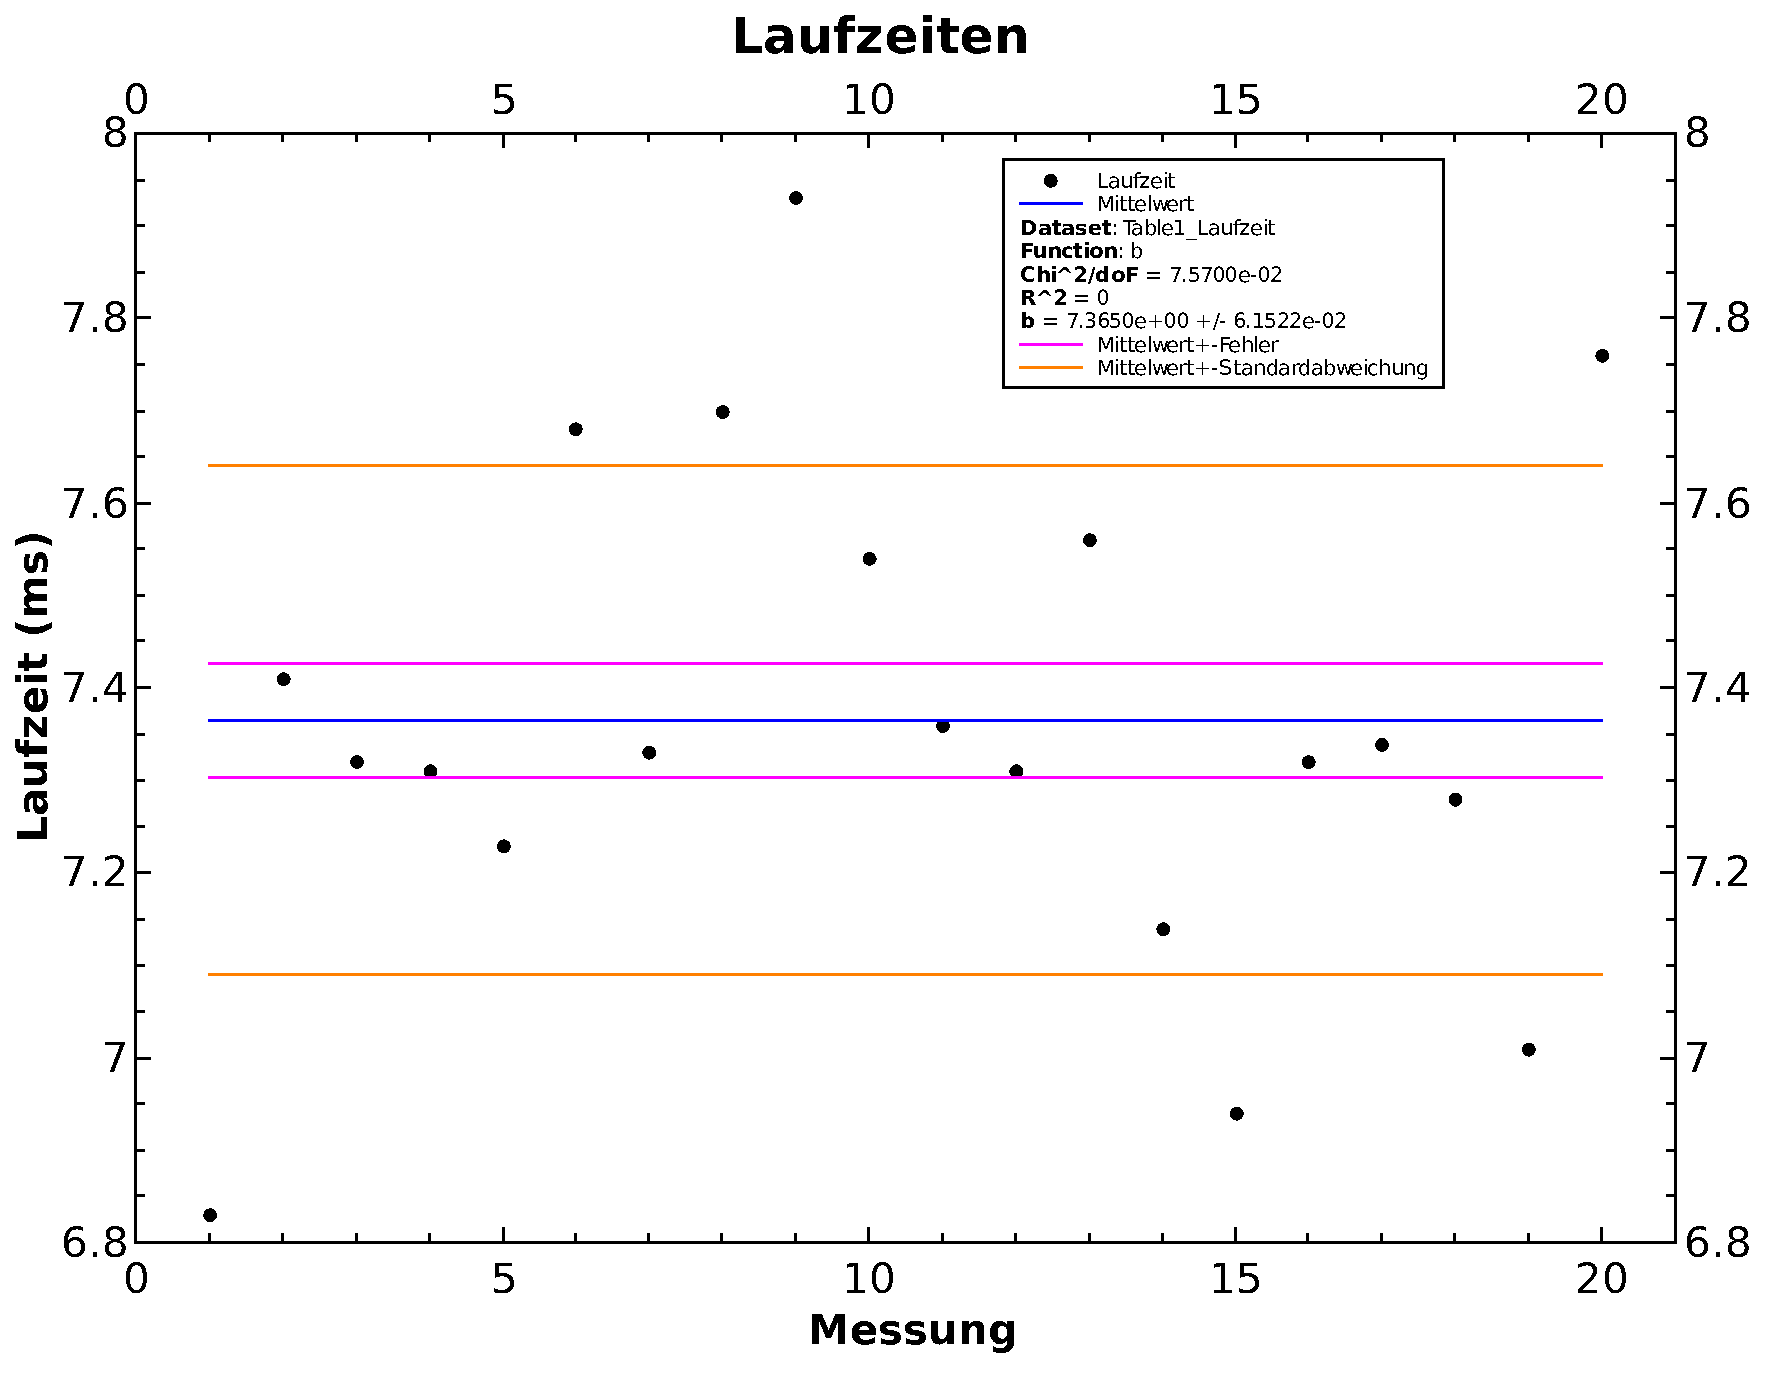
\includegraphics[width=\textwidth]{images/aufgabe1.pdf}
    \caption{Messdaten und Auswertung zum Versuch \emph{Schallgeschwindigkeit}}
    \label{fig:schallgeschwindigkeit}
\end{figure}

13 der  20 Messpunkte (also 65\%)  liegen innerhalb des Mittelwerts  $\pm$ die
Standardabweichung,  was  ziemlich  nahe  beim  theoretischen  Wert  von  68\%
ist. Mit  einer gr\"osseren  Anzahl  Messungen sollte  sich  dieser Wert  noch
besser an 68\% ann\"ahern.

\clearpage
% **************************************************************************** %
\subsection{Aufgabe 2: Eisengehalt}
% **************************************************************************** %

\subsubsection{Daten}
\begin{center}
\begin{tabular}{rrr}
    \toprule
    Messung & Eisengehalt (\%) & absoluter Fehler (\%) \\
    \midrule
    1 & 20.3 & 1.2 \\
    2 & 21.9 & 1.3 \\
    3 & 21.1 & 1.1 \\
    4 & 19.6 & 0.8 \\
    5 & 19.9 & 1.3 \\
    6 & 18.0 & 1.3 \\
    7 & 19.4 & 1.0 \\
    8 & 22.2 & 2.0 \\
    9 & 21.6 & 0.8 \\
    \bottomrule
\end{tabular}
\end{center}

\subsubsection{Einfacher Mittelwert}

Der einfache Mittelwert ergibt sich als:
\begin{equation}
    \overline{x} = \frac{1}{9}\sum_{i=1}^9 x_i = \SI{20.44}{\percent}
\end{equation}

Mit dem zugeh\"origen Fehler:
\begin{equation}
    s_{\overline{x}} = \sqrt{\frac{\sum_1^9(x_i-\overline{x})^2}{9 \cdot 8}} = \SI{0.46}{\percent}
\end{equation}


\subsubsection{Gewichteter Mittelwert}

Der gewichtete Mittelwert errechnet sich gem\"ass:
\begin{equation}
    \overline{x} = \frac{\sum_1^9 g_{\overline{x_i}} \cdot x_i}{\sum_1^9 g_{\overline{x_i}}} = \frac{156.24}{7.67} \si{\percent} = \SI{20.37}{\percent}
\end{equation}

Der zugeh\"orige Fehler Betr\"agt:
\begin{equation}
    s_{\overline{x}} = \frac{1}{\sum_1^9 g_{\overline{x_i}}} = \SI{0.36}{\percent}
\end{equation}

\clearpage
\subsubsection{QtiPlot}
\begin{figure}[th!]
    \centering
    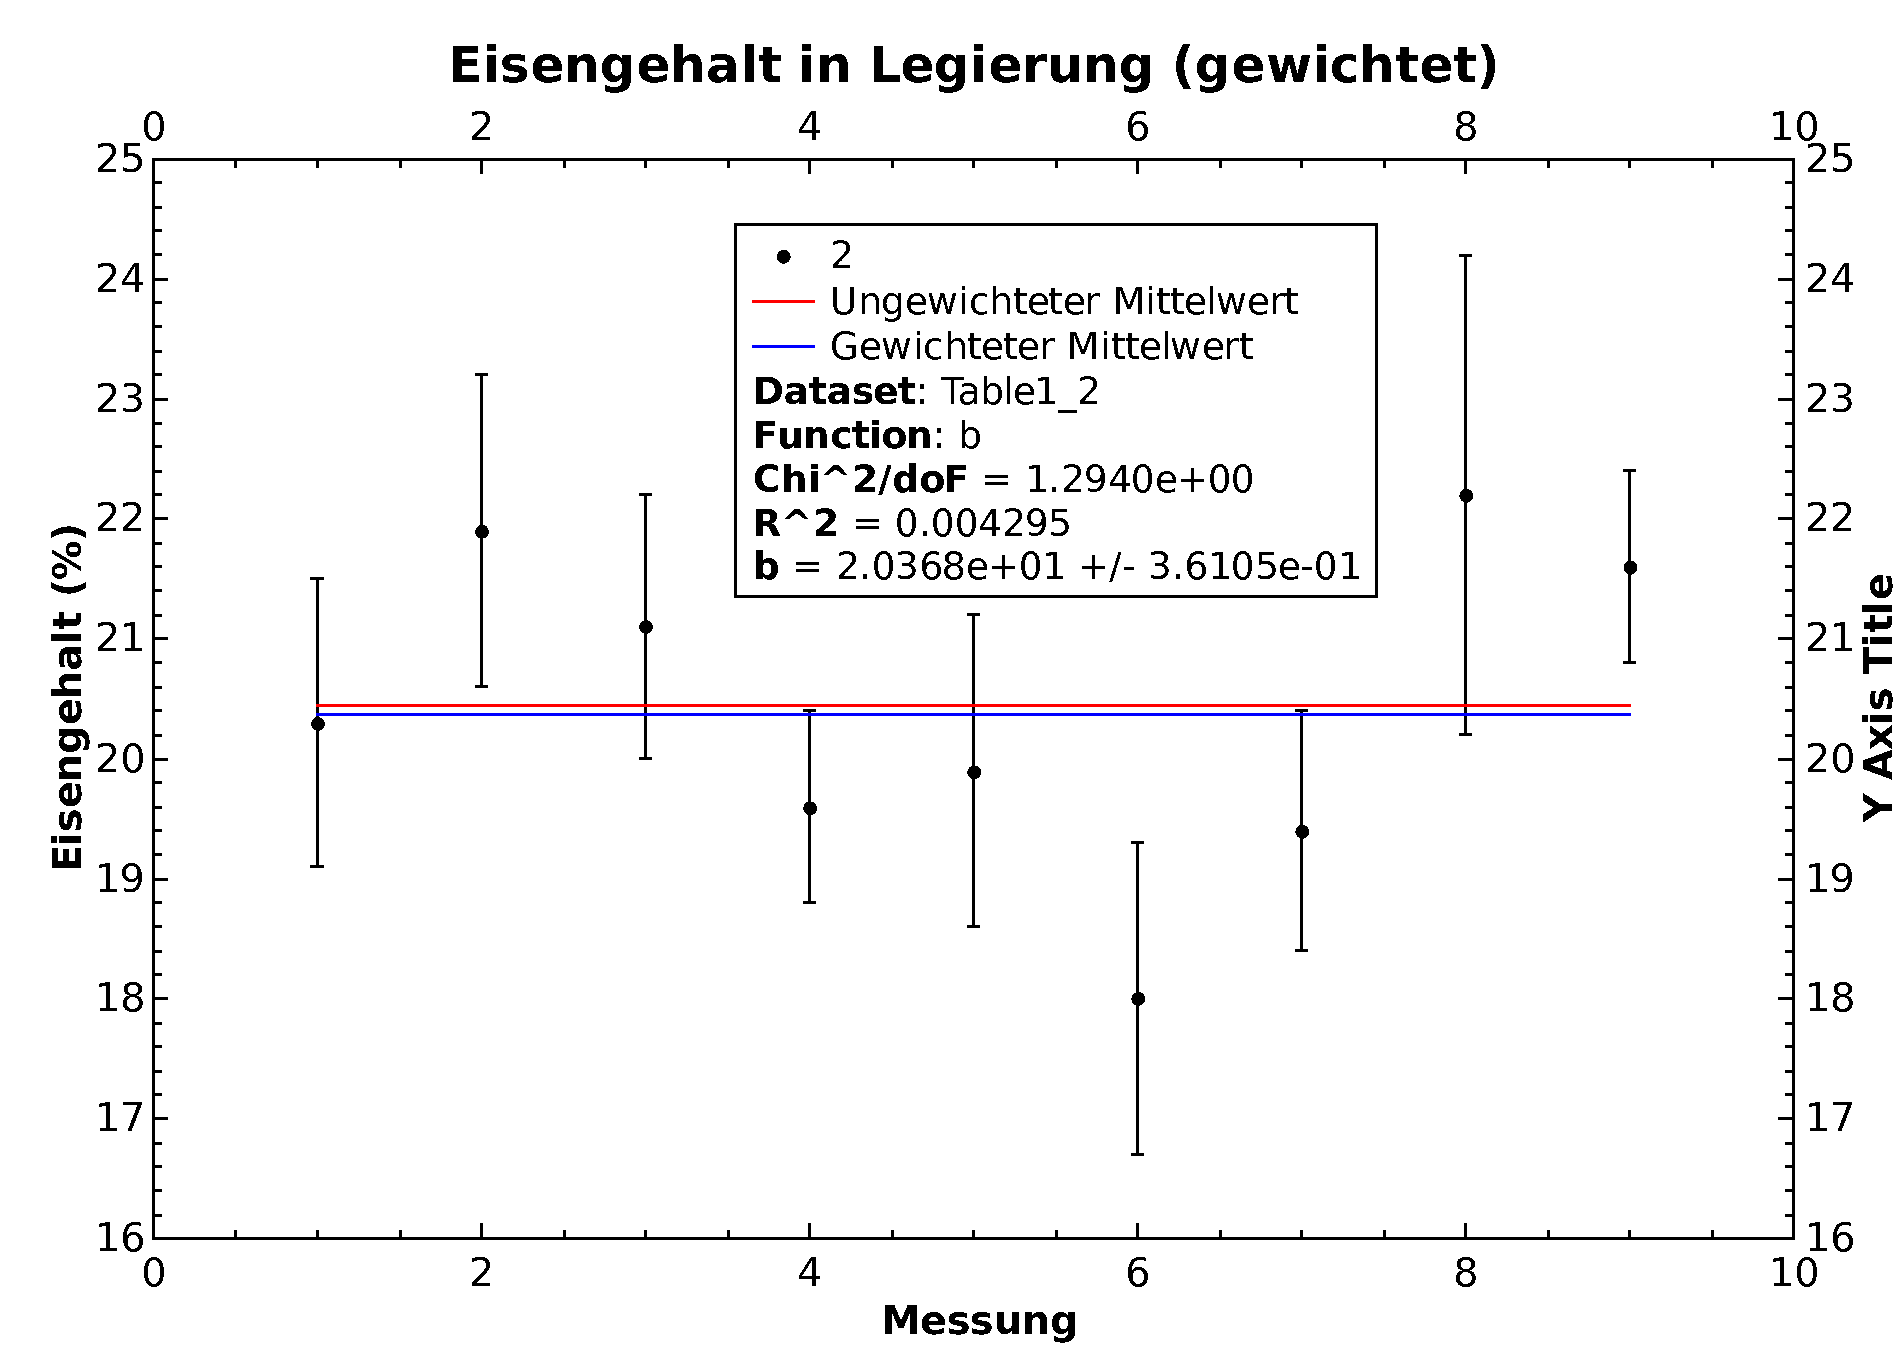
\includegraphics[width=\textwidth]{images/aufgabe2.pdf}
    \caption{Messdaten mit Fehlerbalken, gewichteter und ungewichteter Mittelwert zum Versuch \emph{Eisengehalt}}
    \label{fig:eisengehalt}
\end{figure}

\clearpage
% **************************************************************************** %
\subsection{Aufgabe 3: Federkonstante}
\label{subsec:federkonstante}
% **************************************************************************** %

\subsubsection{Daten}

\begin{center}
\begin{tabular}{rr}
    \toprule
    F (N) & z (m) \\
    \midrule
    3.83  & 0.20 \\
    7.79  & 0.35 \\
    8.08  & 0.42 \\
    9.7   & 0.46 \\
    10.58 & 0.51 \\
    12.33 & 0.54 \\
    12.23 & 0.59 \\
    14.43 & 0.67 \\
    15.51 & 0.71 \\
    17.09 & 0.80 \\
    \bottomrule
\end{tabular}
\end{center}

\subsubsection{Rechnung mittels Tabellenkalkulation}

Zum  Vergleich mit  dem  Resultat  des Taschenrechners  und  QtiPlot sei  hier
noch eine  lineare Regression mit  Tabellenkalkulationsprogramm durchgef\"uhrt
gem\"ass der Anleitung im  deutschen Wikipedia-Artikel zur linearen Regression
\cite{ref:wikipedia:lineareRegression}.

\begin{tabular}{rrrrrrrr}
    \toprule
                F (N)&z (m)&&&&&& $\hat{F}(N)$ \\
    \midrule
             $y_i$      & $x_i$      &  $y_i-\overline{y}$ & $x_i-\overline{x} $ & $(y_i-\overline{y})(x_i-\overline{x})$ & $(y_i-\overline{y})^2$ & $(x_i-\overline{x})^2$ & $ \hat{y}  $ \\
    \midrule
               3.83&        0.20&              -7.33  &              -0.32  &                 2.38                   &        53.68           &         0.11           &  3.82 \\
               7.79&        0.35&              -3.37  &              -0.17  &                 0.59                   &        11.34           &         0.03           &  7.21 \\
               8.08&        0.42&              -3.08  &              -0.10  &                 0.32                   &         9.47           &         0.01           &  8.79 \\
               9.70&        0.46&              -1.46  &              -0.06  &                 0.09                   &         2.12           &         0.00           &  9.69 \\
              10.58&        0.51&              -0.58  &              -0.01  &                 0.01                   &         0.33           &         0.00           &  10.82 \\
              12.33&        0.54&               1.17  &               0.02  &                 0.02                   &         1.38           &         0.00           &  11.50 \\
              12.23&        0.59&               1.07  &               0.07  &                 0.07                   &         1.15           &         0.00           &  12.62 \\
              14.43&        0.67&               3.27  &               0.15  &                 0.47                   &        10.71           &         0.02           &  14.43 \\
              15.51&        0.71&               4.35  &               0.19  &                 0.81                   &        18.95           &         0.03           &  15.33 \\
              17.09&        0.80&               5.93  &               0.28  &                 1.63                   &        35.20           &         0.08           &  17.36 \\
    \midrule
             111.57&        5.25&               0.00  &               0.00  &                 6.40                   &       144.33           &         0.29           & Summen \\
    \midrule
              11.16&        0.52&&&&&& Durchschnitte \\
    \bottomrule
\end{tabular}

Die Steigung der Regressionsgeraden errechnet sich als:
\begin{equation}
    k = \frac{\sum_{i=1}^{10}(x_i-\overline{x})(y_i-\overline{y})}{\sum_{i=1}^{10}(x_i-\overline{x})^2} = \frac{144.33}{6.4} \si{\newton\per\meter} = \SI{22.57}{\newton\per\meter}
\end{equation}

Den Achsenabschnitt $F_0$ erh\"alt man aus:
\begin{equation}
    F_0 = \overline{y} - k \cdot \overline{x} = \SI{11.16}{\newton} - \SI{22.57}{\newton\per\meter} \cdot \SI{0.52}{\meter} = \SI{-0.69}{\newton}
\end{equation}

Die empirische Korrelation betr\"agt:
\begin{equation}
    r_{xy} = \frac{\sum_{1}^{10}(x_i - \overline{x}) \cdot (y_i - \overline{y})}{\sqrt{\sum_{1}^{10}(x_i-\overline{x})^2 \cdot \sum_{1}^{10}(y_i-\overline{y})^2}}
           = \frac{6.40}{\sqrt{144.33 \cdot 0.29}} = 0.99364
\end{equation}

Das Bestimmtheitsmass betr\"agt:
\begin{equation}
    R^{2} = r_{xy}^2 = 0.98732
\end{equation}

\subsubsection{Taschenrechner}

Ergebnisse    ermittelt   mittels    TI-89    und    Anleitung   aus    Quelle
\cite{ref:ti89:regression} (um Einheiten erg\"anzt).

\begin{gather*}
    F = k \cdot z + F_0 \\
    k = \SI{22.280962}{\newton\per\meter} \\
    F_0 = \SI{-0.540505}{\newton} \\
    corr = 0.993638 \\
    R^2 = 0.987316
\end{gather*}

\subsubsection{QtiPlot}
\begin{figure}[th!]
    \centering
    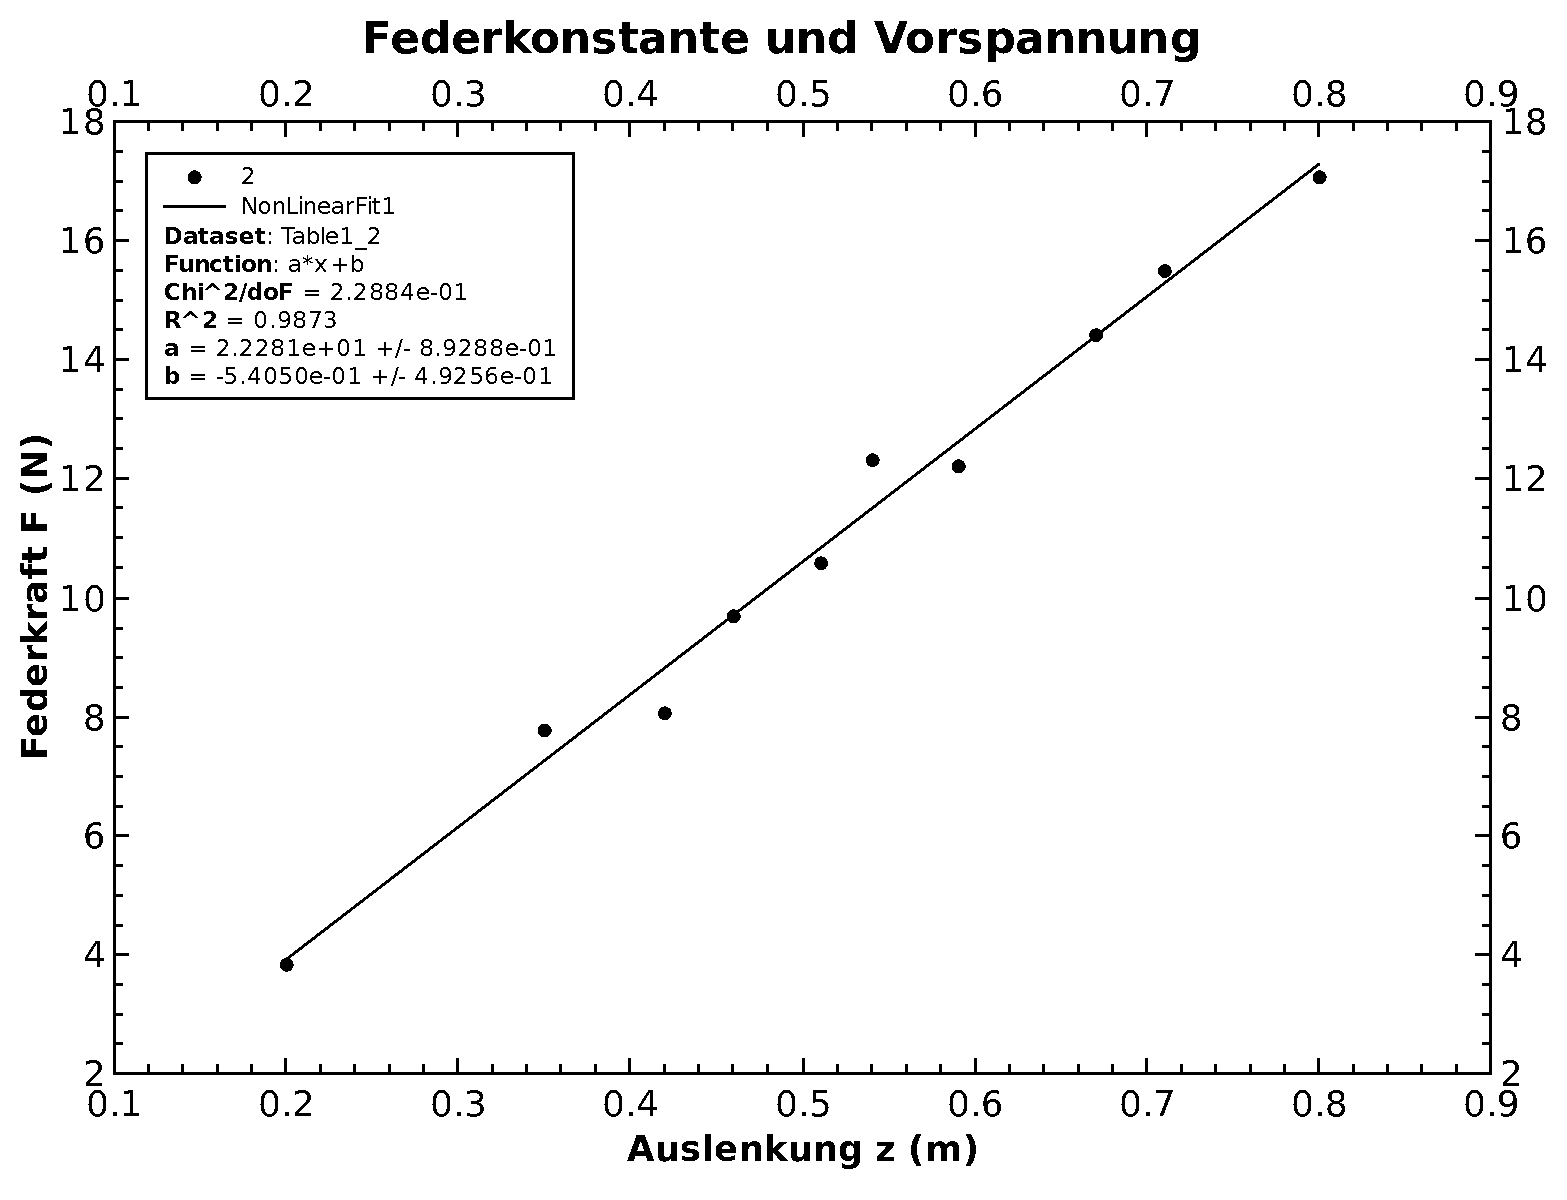
\includegraphics[width=.8\textwidth]{images/aufgabe3-1.pdf}
    \caption{Regressionsgerade mit Messpunkten zu Aufgabe \emph{Federkonstante}}
    \label{fig:federkonstante1}
\end{figure}
\begin{figure}[th!]
    \centering
    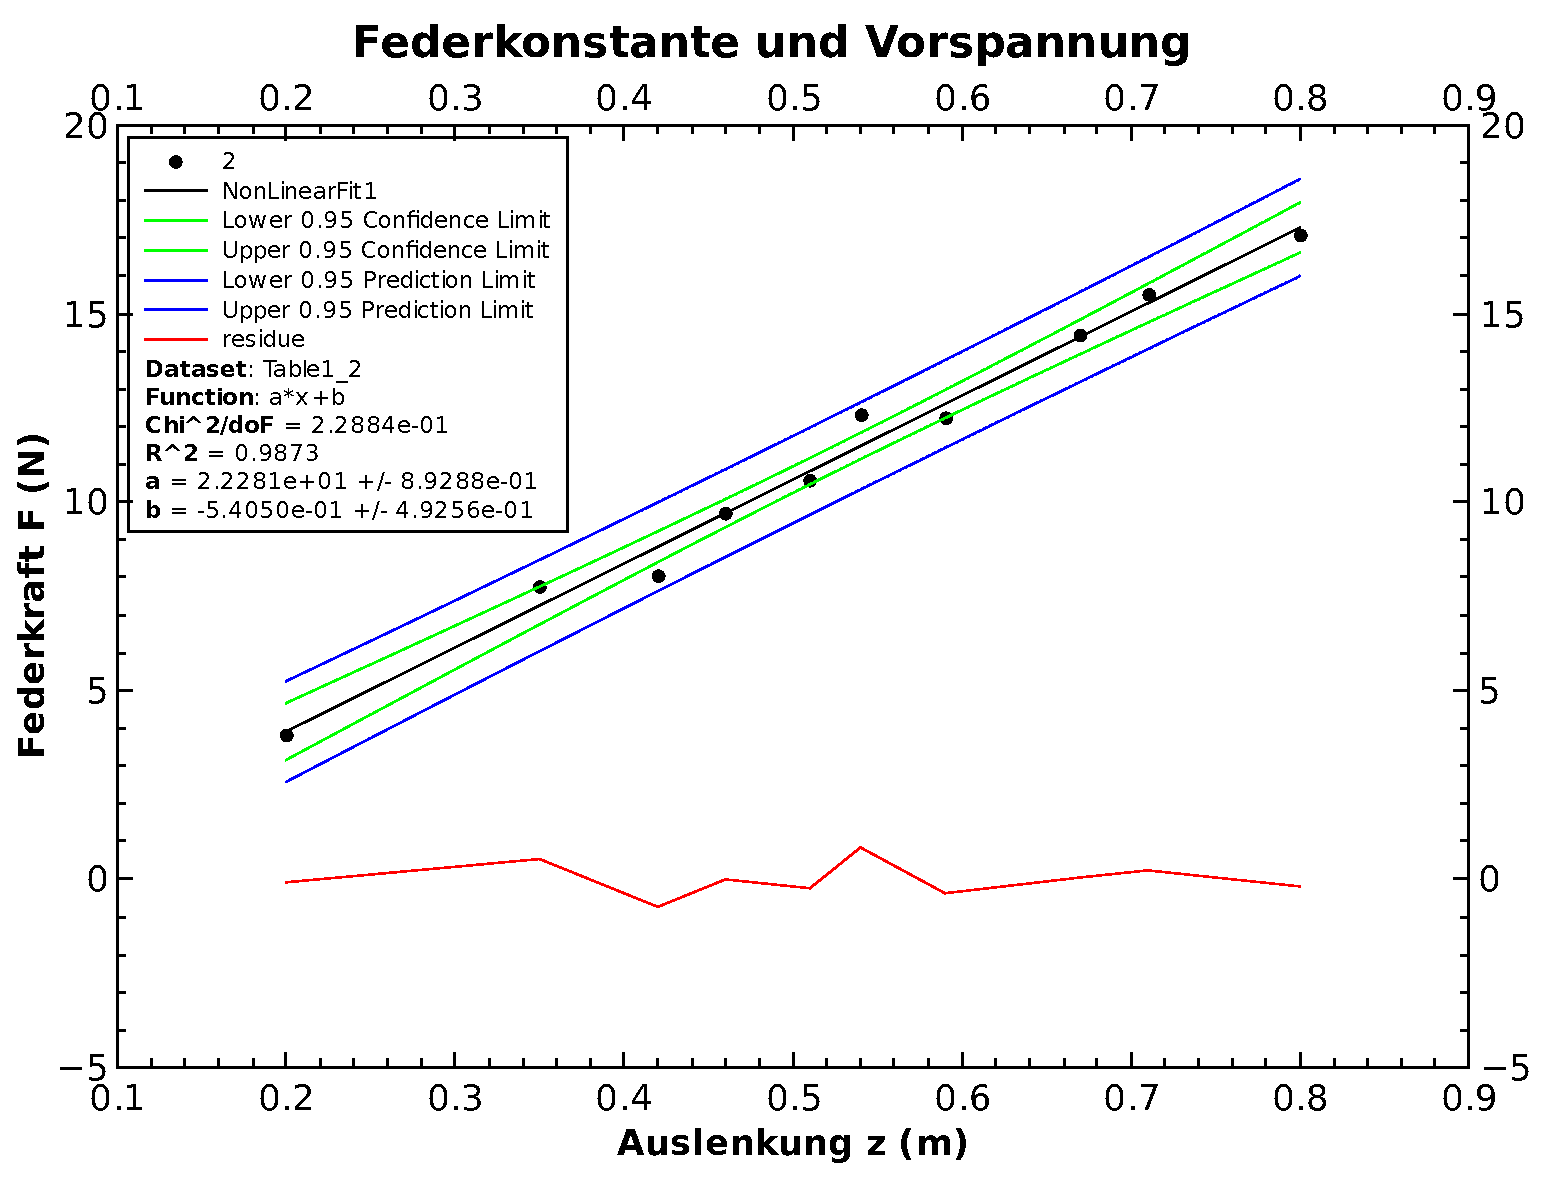
\includegraphics[width=.8\textwidth]{images/aufgabe3-2.pdf}
    \caption{Regressionsgerade mit Messpunkten, 95\% Confidence Band, Prediction Band und Residuals zu Aufgabe \emph{Federkonstante}}
    \label{fig:federkonstante2}
\end{figure}
\begin{figure}[th!]
    \centering
    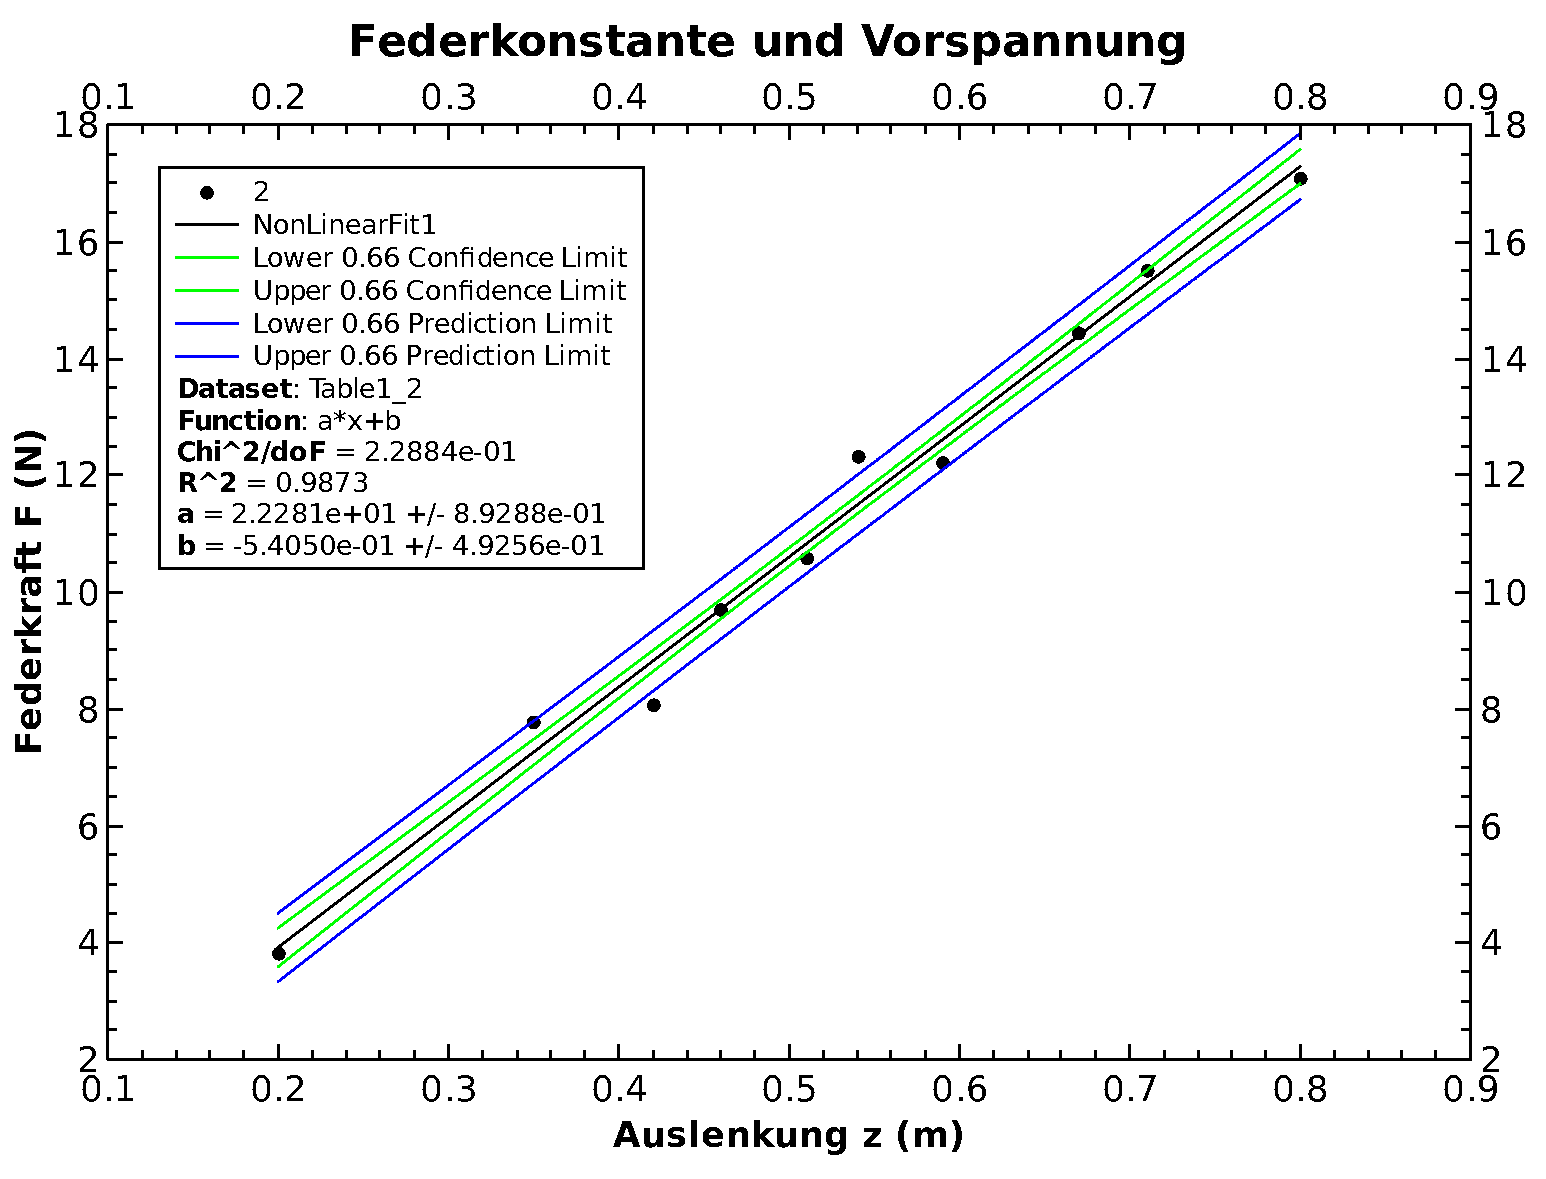
\includegraphics[width=.8\textwidth]{images/aufgabe3-3.pdf}
    \caption{Regressionsgerade mit Messpunkten, 66\% Confidence Band und Prediction Band zu Aufgabe \emph{Federkonstante}}
    \label{fig:federkonstante3}
\end{figure}

\clearpage
% **************************************************************************** %
\subsection{Aufgabe 4: Pendel}
\label{subsec:pendel}
% **************************************************************************** %

\subsubsection{Theorie}

Die  ged\"ampfte Schwingung  eines  Pendels  kann folgendermassen  beschrieben
werden:
\begin{equation}
    y(t) = A \cdot exp(-\Gamma \cdot t) \cdot sin(2 \cdot \pi \cdot f \cdot t - \delta) + y_0
    \label{eq:pendulum}
\end{equation}

Nun  soll eine  Funktion mittels  QtiPlot  auf die  unten stehenden  Messdaten
gefittet werden, um die Parameter dieser Gleichung zu bestimmen.

Dabei wird von QtiPlot eine nichtlineare Regression ausgef\"uhrt. Es muss also
das Minimum der folgenden Funktion gefunden werden:

\begin{equation}
    \label{eq:chi}
    \chi^2(a_1,a_2,a_3,...,a_N) = \sum_1^N \frac{ [y_i - f(a_1,a_2,a_3,...,a_N) ]^2}{\sigma_i}
\end{equation}

$\sigma_i$ sind dabei die Fehler der einzelnen Messungen $y_i$.

Es  gilt  nun,  geeignete  Startwerte f\"ur  die  nichtlineare  Regression  zu
finden. Ansonsten wird  QtiPlot entweder  kein Resultat  erhalten (Algorithmus
konvergiert nicht) oder ein Nebenminimum der $\chi^2$-Funktion finden, welches
nicht die bestm\"ogliche Ann\"aherung an die gesuchte Gesetzm\"assigkeit ist.

\subsubsection{Messdaten}
(von Aufgabenblatt kopiert)

\begin{center}
    \begin{tabular}{*{12}{c}}
        \toprule
        $t(s)$  &  $y(m)$   &  $t(s)$   &  $y(m)$   &  $t(s)$  &  $y(m)$    &  $t(s)$   & $y(m)$    &  $t(s)$   &  $y(m)$   &  $t(m)$   &  $y(m)$ \\
        \midrule
        0.5     & -0.418    & 8.0       & 0.594     & 15.5     & -0.577     & 23.0      & 0.417     & 30.5      & -0.132    & 38.0      & 0.152   \\
        1.0     & -0.07     & 8.5       & 0.632     & 16.0     & -0.48      & 23.5      & 0.423     & 31.0      & -0.123    & 38.5      & 0.058   \\
        1.5     & 0.082     & 9.0       & 0.435     & 16.5     & -0.414     & 24.0      & 0.45      & 31.5      & -0.075    & 39.0      & 0.193   \\
        2.0     & 0.19      & 9.5       & 0.366     & 17.0     & -0.46      & 24.5      & 0.389     & 32.0      & -0.373    & 39.5      & 0.070   \\
        2.5     & 0.494     & 10        & 0.123     & 17.5     & -0.187     & 25.0      & 0.488     & 32.5      & -0.146    & 40.0      & 0.235   \\
        3.0     & 0.566     & 10.5      & 0.064     & 18.0     & -0.171     & 25.5      & 0.317     & 33.0      & -0.176    & 40.5      & 0.084   \\
        3.5     & 0.753     & 11.0      & -0.084    & 18.5     & -0.03      & 26.0      & 0.344     & 33.5      & -0.193    & 41.0      & 0.248   \\
        4.0     & 0.913     & 11.5      & -0.152    & 19.0     & -0.072     & 26.5      & 0.363     & 34.0      & -0.138    & 41.5      & 0.319   \\
        4.5     & 0.869     & 12.0      & -0.299    & 19.5     & -0.011     & 27.0      & 0.218     & 34.5      & -0.259    & 42.0      & 0.052   \\
        5.0     & 0.977     & 12.5      & -0.506    & 20.0     & 0.082      & 27.5      & 0.084     & 35.0      & -0.078    & 42.5      & 0.159   \\
        5.5     & 0.956     & 13.0      & -0.479    & 20.5     & 0.109      & 28.0      & 0.113     & 35.5      & 0.018     & 43.0      & 0.134   \\
        6.0     & 0.996     & 13.5      & -0.576    & 21.0     & 0.25       & 28.5      & 0.166     & 36.0      & -0.059    & 43.5      & 0.079   \\
        6.5     & 0.971     & 14.0      & -0.662    & 21.5     & 0.404      & 29.0      & 0.02      & 36.5      & 0.056     & 44.0      & 0.097   \\
        7.0     & 0.827     & 14.5      & -0.498    & 22.0     & 0.272      & 29.5      & -0.032    & 37.0      & 0.004     & 44.5      & 0.162   \\
        7.5     & 0.784     & 15.0      & -0.654    & 22.5     & 0.317      & 30.0      & 0.011     & 37.5      & 0.042     & 45.0      & 0.030   \\
        \bottomrule
    \end{tabular}
\end{center}

\clearpage
\subsubsection{QtiPlot}

Die Pendelgleichung wurde in QtiPlot folgendermassen definiert:

\begin{verbatim}
    A*exp(-G*x)*sin(2*pi*f*x-d)+y0
\end{verbatim}

Die Startwerte wurden mit folgender Methodik bestimmt:
\begin{itemize}
    \item
        $A = 1$: Anhand des Funktionswertes des ersten Ausschlages des Pendels
        abgesch\"atzt.
    \item
        $\Gamma  =  ln  \left(\frac{A_1}{A_2}   \right)  \cdot  \frac{1}{T}  =
        ln  \left(\frac{1}{0.5}   \right)  \cdot   \frac{1}{20}  =   0.035  $:
        Die   Abklingkonstante  $\Gamma$   wurde  abgesch\"atzt   mittels  des
        logarithmischen   Dekrements   und   der  Periode. Dabei   ist   $A_1$
        die  Amplitude   des  ersten  Schwingvorgangs,  $A_2$   die  Amplitude
        des  2. Schwingvorgangs   und  $T$  die  Periode   der  unterliegenden
        Sinus-Schwingung. Nat\"urlich   sind  all   diese   Werte  eher   grob
        aus   dem  Scatter-Plot   abgelesen  und   nicht  hochpr\"azise   (was
        aber  f\"ur  diesen  Schritt   auch  nicht  notwendig  ist). Genaueres
        kann     in     den     Quellen~\cite{ref:wikipedia:abklingkonstante},
        ~\cite{ref:wikipedia:periode}   und~\cite{ref:wikipedia:logarithmDekr}
        gefunden werden.
    \item
        Der  Nulldurchgang der  ersten Schwingung  liegt ungef\"ahr  bei einer
        Sekunde, wie  man auf dem Scatter-Plot  erkennen kann. Dies entspricht
        der Forderung, dass  $sin(2 \cdot \pi \cdot f  \cdot \SI{1}{\second} -
        \delta) = 0$ ist,  bzw. weil $sin(0) = 0$, muss  gelten:  $2 \cdot \pi
        \cdot f \cdot \SI{1}{\second} -  \delta = 0$. Aufgel\"ost ergibt dies:
        $\delta =  2 \cdot  \pi \cdot  f \cdot \SI{1}{\second}  = 2  \cdot \pi
        \cdot \frac{1}{\SI{20}{\second}} \cdot \SI{1}{\second} = 0.31$.
    \item
        Die Periode  der Sinus-Schwingung wird  aus den Peaks der  zwei ersten
        Schwingungen  auf  ungef\"ahr  20   Sekunden  gesch\"atzt,  womit  man
        f\"ur  die Frequenz  $\frac{1}{\SI{20}{\second}} =  \SI{0.05}{\hertz}$
        erh\"alt.
    \item
        Der Offset $y_0$ wird vorerst auf null gesetzt.
\end{itemize}

Somit sind die Startwerte bestimmt und werden wie folgt in QtiPlot eingesetzt:
\begin{verbatim}
    A = 1
    G = 0.035
    f = 0.05
    d = 0.31
    y0 = 0
\end{verbatim}

Dies liefert:

\begin{figure}[th!]
    \centering
    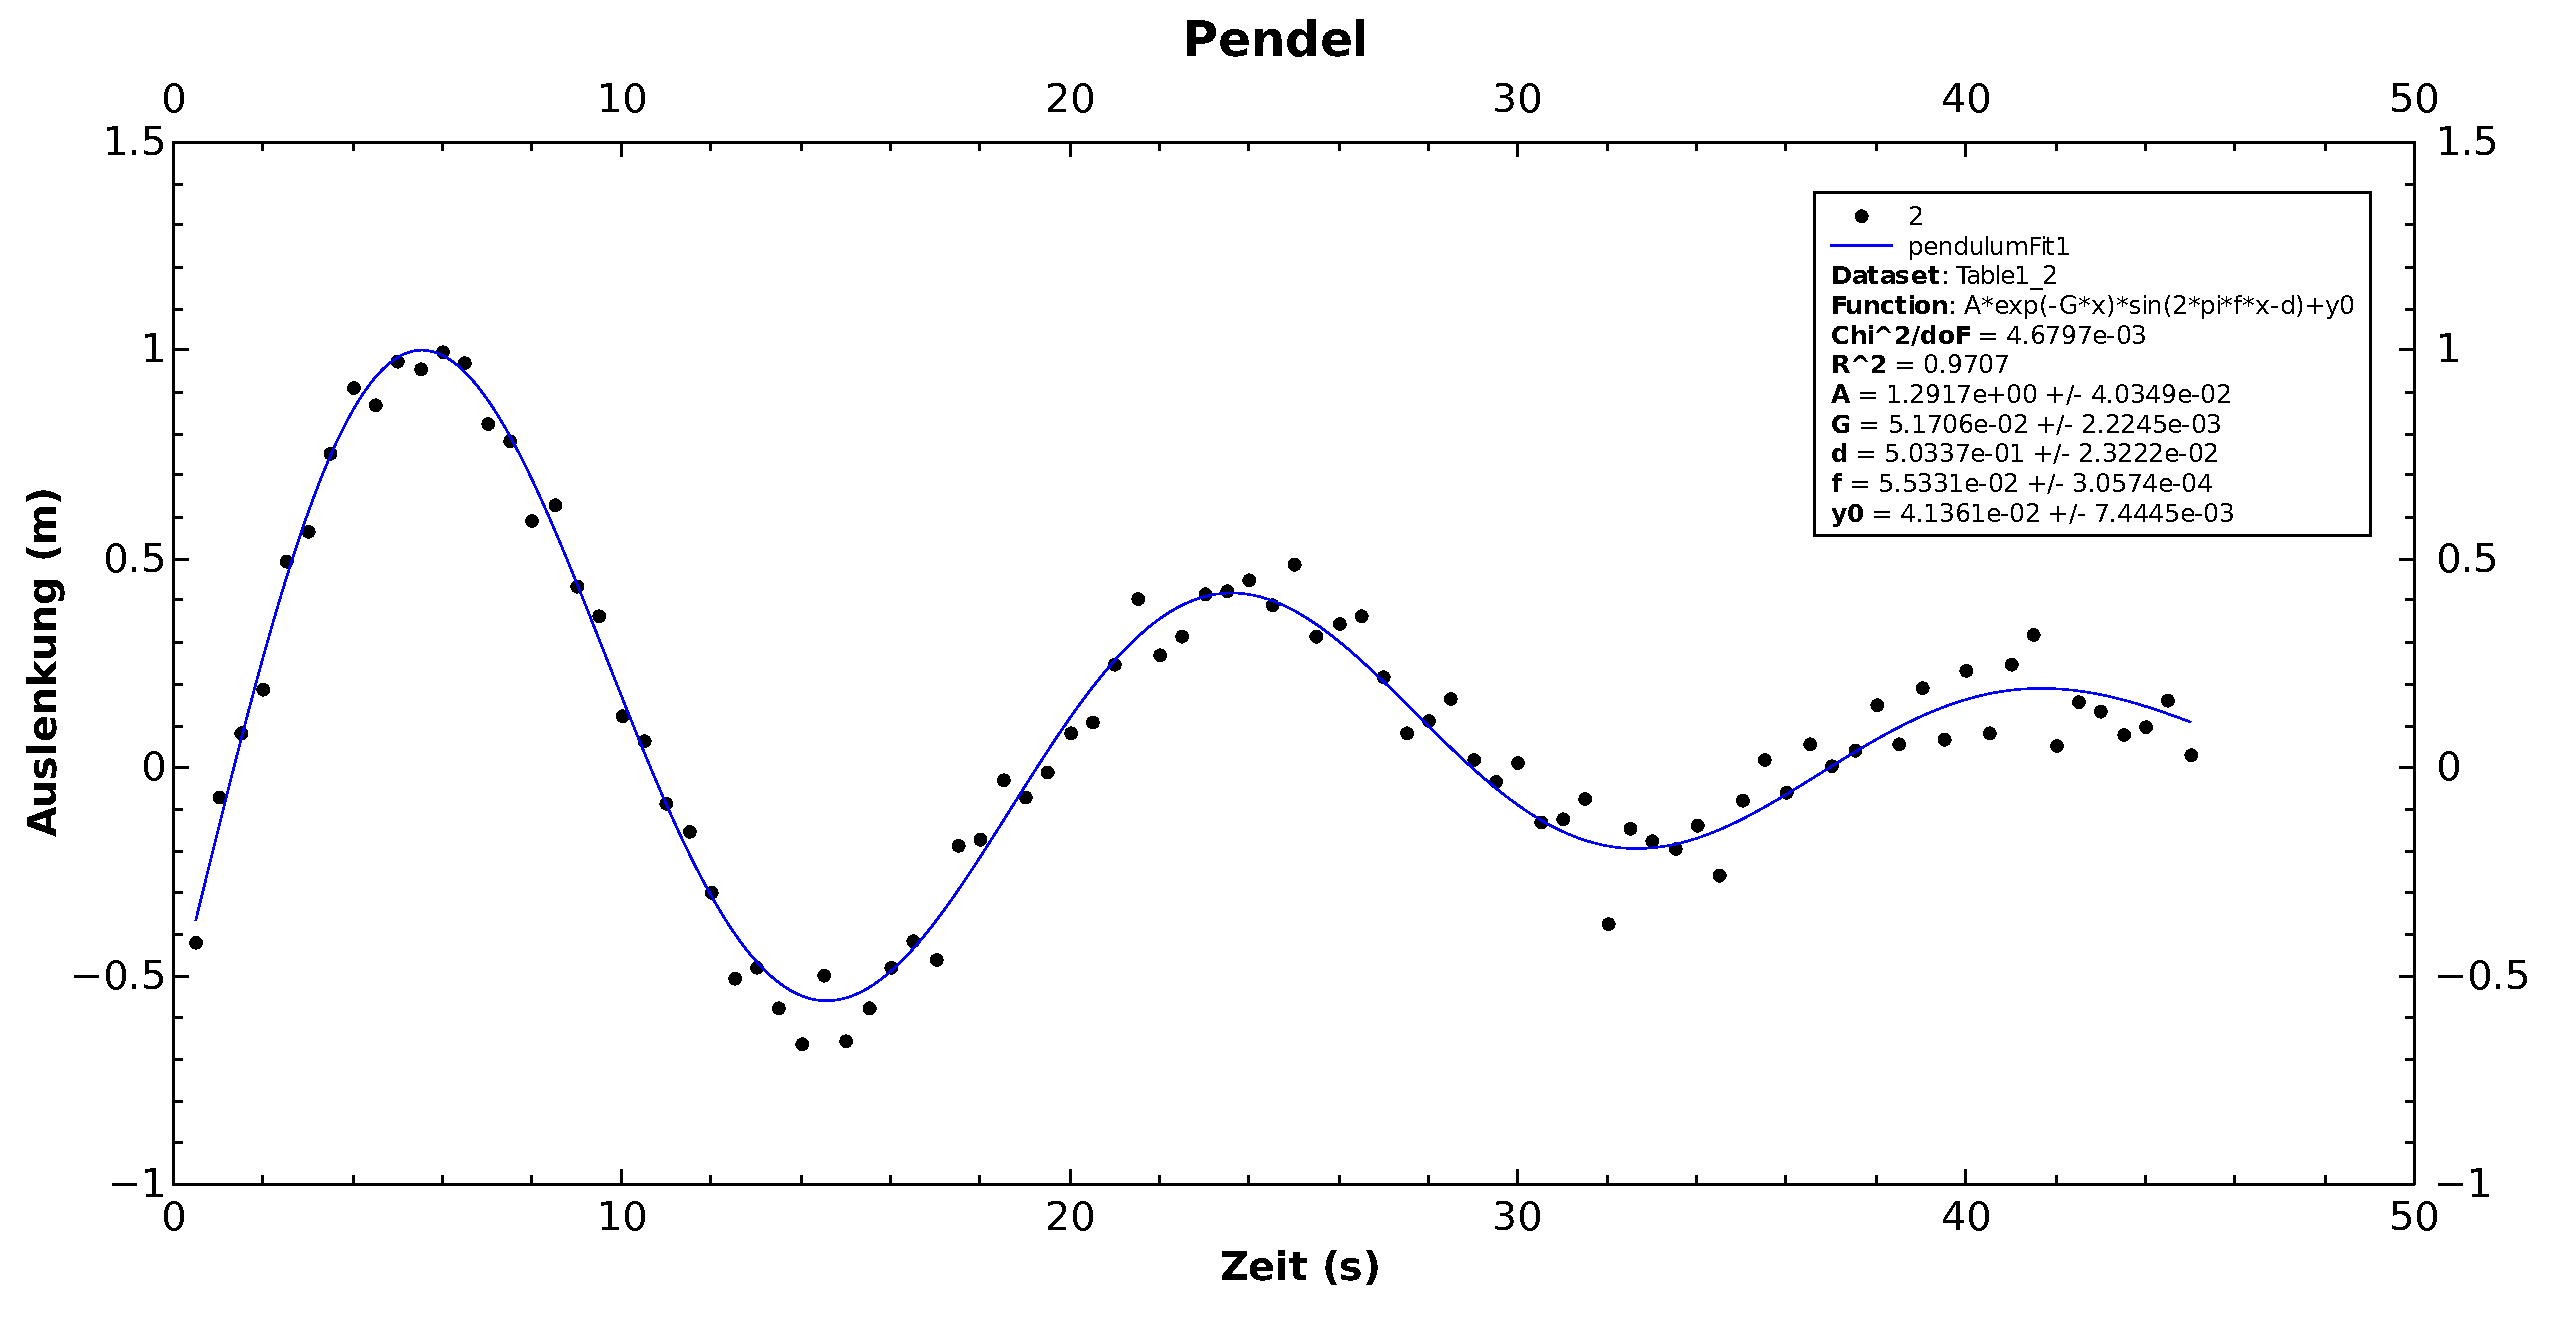
\includegraphics[width=\textwidth]{images/aufgabe4.pdf}
    \caption{Fit zur Aufgabe \emph{Pendel}, mit den gesuchten Gleichungsparametern (siehe Legende)}
    \label{fig:pendulum}
\end{figure}

Die  von  QtiPlot bestimmten  Gleichungsparameter  sind  gem\"ass Legende  aus
Abbildung \ref{fig:pendulum} somit (mit Einheiten erg\"anzt):
\begin{align*}
    A      & = \SI[separate-uncertainty  = true]{ 1.2917   \pm 0.040349}{\meter} \\
    \Gamma & = \SI[separate-uncertainty  = true]{-0.051706 \pm 0.0022245}{\per\second} \\
    f      & = \SI[separate-uncertainty  = true]{ 0.05331  \pm 0.00030574}{\hertz} \\
    \delta & = \num[separate-uncertainty = true]{ 0.50337  \pm 0.023222} \\
    y_0    & = \SI[separate-uncertainty  = true]{ 0.041361 \pm 0.0074445}{\meter}
\end{align*}

Sinnvoll gerundet und mit Einheiten in Gleichung~\ref{eq:pendulum} eingesetzt:
\begin{align*}
    y(t)   & = A \cdot exp(-\Gamma \cdot t) \cdot sin(2 \cdot \pi \cdot f \cdot t - \delta) + y_0 \\
           & =     \SI[separate-uncertainty = true]{1.29 \pm 0.04}{\meter}
           \cdot exp\left(\SI[separate-uncertainty = true]{-0.052 \pm 0.002}{\per\second}\right) \\
           & \cdot sin\left(2\pi \cdot \SI[separate-uncertainty = true]{0.0533 \pm 0.0003}{\hertz} \cdot t - \num[separate-uncertainty = true]{0.50 \pm 0.02}\right) \\
           & + \SI[separate-uncertainty = true]{0.041 \pm 0.007}{\meter}
\end{align*}


\clearpage
% **************************************************************************** %
\subsection{Aufgabe 5: RC-Glied (Tiefpass)}
% **************************************************************************** %

Es soll das Verhalten eines Tiefpasses untersucht werden:
\begin{figure}[th!]
    \centering
    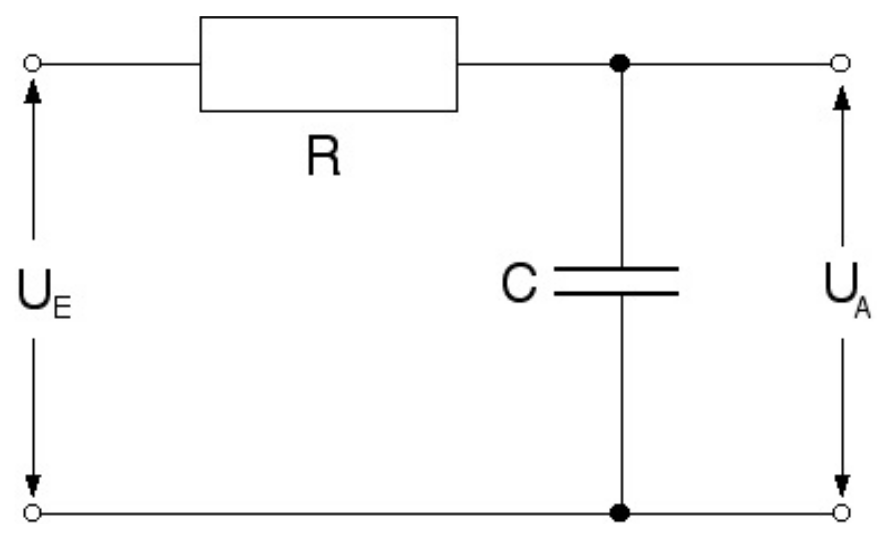
\includegraphics[width=.4\textwidth]{images/rc-glied.png}
    \caption{Tiefpass. \textbf{Quelle}: Versuchsunterlagen ``Auswertung mit Computer'', p.6}
    \label{fig:rcGlied}
\end{figure}

\subsubsection{Versuchsdurchf\"uhrung und Messdaten}

Aus der Aufgabenstellung \"ubernommen:

\begin{quote}
Am  Eingang des  RC-Tiefpasses wurde  eine sinusf\"ormige  Wechselspannung mit
konstanter Spannung $U_E = \SI{4}{\volt}_{pp}$  (Peak-Peak = PP) und variabler
Frequenz angelegt. Sodann  wurde die  Ausgangsspannung $U_A$  (PP-Werte) sowie
die Phasenverschiebung  $\varphi$ in Funktion  der Frequenz f mit  Hilfe eines
Kathodenstrahloszilloskopes  (KO) gemessen. Der  Widerstand  R wurde  zu $R  =
\SI{500}{\ohm}$ bestimmt. Dabei wurde untenstehendes Messprotokoll erstellt.
\\
\begin{center}
        \begin{tabular}{rrrr}
            \toprule
            \multicolumn{3}{l}{Messprotokoll ``Tiefpass''} \\
            \multicolumn{3}{l}{Datum: 1. Okt. 1999} \\
            \multicolumn{3}{l}{Versuchsleiterin: Ruth Metzler} \\
            \midrule
            $f(Hz)$  &  $U_a (V)$    &  $\varphi (\degree)$ & $\varphi (rad)$ \\
            \midrule
            100      & 4.000        & -3.24 &  -0.05655 \\
            500      & 3.800        & -16.9 &  -0.295   \\
            1000     & 3.300        & -31.3 &  -0.5463  \\
            1500     & 2.800        & -43.6 &  -0.761   \\
            5000     & 1.140        & -72.4 &  -1.264   \\
            10000    & 0.580        & -82.5 &  -1.44    \\
            100000   & 0.075        & -90.0 &  -1.571   \\
            1592     & 2.700        & -44.0 &  -0.7679  \\
            \bottomrule
        \end{tabular}
        \label{tab:rc}
\end{center}
\end{quote}

\textbf{Anmerkung}: Das Messprotokoll wurde noch um  eine Spalte mit der Phase
in radians erg\"anzt, welche in QtiPlot f\"ur die Auswertung benutzt wird.


\subsubsection{Funktionsgleichungen}
Ausgangs- und Eingangsspannung verhalten sich wie folgt zueinander:
\begin{align}
    U_A & = \frac{X_C}{\sqrt{X_C^2+R^2}} \cdot U_E \\
                    & = \frac{1}{\omega \cdot C \cdot \sqrt{\frac{1}{(\omega \cdot C)^2} + R^2}} \cdot U_E \\
                    & = \frac{1}{\sqrt{1+(\omega \cdot C \cdot R)^2}} \cdot U_E
    \label{eq:rc:uaue}
\end{align}

F\"ur   die  Phase   zwischen   Aus-  und   Eingangsspannung  gilt   folgender
Zusammenhang:

\begin{equation}
    \varphi = arctan(-\omega R C)
    \label{eq:rc:phi}
\end{equation}

Diese Gleichungen wurden in QtiPlot als folgende Funktionen definiert:

\begin{verbatim}
    1/sqrt(1+(2*pi*x*C*R)^2)*Ue
    atan(-2*pi*x*R*C)
\end{verbatim}


\subsubsection{Startwerte}
\label{subsubsec:rcglied:startwerte}

Die Startwerte f\"ur $U_E$, $C$ und $R$ wurden folgendermassen festgelegt:

\begin{itemize}
    \item
        Der   Widerstand   wurde   gem\"ass    Aufgabenstellung   auf   $R   =
        \SI{500}{\ohm}$ fixiert  und in den Einstellungen  als \emph{constant}
        markiert, damit QtiPlot nicht versucht, diesen Wert zu ``optimieren''.
    \item
        Die    Eingangsspannung   betr\"agt    gem\"ass   den    Angaben   zur
        Versuchsdurchf\"uhrung   $\SI{4}{\volt}$. Sie   wurde  ebenfalls   als
        \emph{constant} definiert.
    \item
        Der   Startwert  f\"ur   die  Kapazit\"at   $C$  wurde   mithilfe eines
        Wertepaares aus der Messwerttabelle gefunden.

        Dazu   wurde   das   Wertepaar   $U_A  =   \SI{2.8}{\volt}$   und   $f
        =   \SI{1500}{\hertz}$   in  Gleichung   \ref{eq:rc:uaue}   eingesetzt
        und   die  Gleichung   nach  $C$   aufgel\"ost.

        Also: $\SI{2.8}{\volt}       =      \frac{1}{\sqrt{1+(2\pi       \cdot
        \SI{1500}{\hertz}    \cdot   C    \cdot   \SI{500}{\ohm})^2}}    \cdot
        \SI{4}{\volt}$ bzw.  $C  = \SI{0.216}{\micro\farad}$ (die quadratische
        Gleichung liefert nat\"urlich auch  den betragsgleichen negativen Wert
        f\"ur $C$,  welcher als  physikalisch unsinnig nicht  weiter verwendet
        wird).

        Es  sei hier  insbesondere  noch erw\"ahnt,  dass sinnvollerweise  ein
        Wertepaar  aus dem  mittleren Bereich  des Scatter-Plots  ausgew\"ahlt
        wird, da dort f\"ur eine  \"Anderung der Frequenz eine viel gr\"ossere
        \"Anderung  der Ausgangsspannung  erreicht wird. Prinzipiell  kann die
        Rechnung mit jedem beliebigen  Wertepaar durchgef\"uhrt werden, jedoch
        ist  bei kleinerem  Hebel zwischen  Frequenz und  Ausgangsspannung die
        Genauigkeit des  erhaltenen Startwertes f\"ur $C$  geringer, und somit
        macht die Verwendung  solcher Wertepaare nicht sehr  viel Sinn solange
        man Wertepaare mit gr\"osserem Hebel zur Verf\"ugung hat (siehe hierzu
        auch Abbildung \ref{fig:rcglied:spannung}).
\end{itemize}

In QtiPlot wurden somit folgende Werte als Startwerte eingesetzt:

\begin{verbatim}
    C = 2.16e-7
    R = 500 (constant)
    Ue = 4 (constant)
\end{verbatim}

F\"ur  den Fit  der  Phase wurden  ebenfalls  diese Werte  f\"ur  $C$ und  $R$
verwendet,  $U_E$ wurde  daf\"ur nat\"urlich  nicht ben\"otigt,  da es  in der
Formel f\"ur $\varphi$ nicht vorkommt.

\clearpage
\subsubsection{QtiPlot}

Der Fit  f\"ur den Zusammenhang  zwischen Ausgangsspannugn $U_A$  und Frequenz
$f$  ist  in  Abbildung  \ref{fig:rcglied:spannung} zu  sehen. Der  Fit  f\"ur
Phase  $\varphi$ und  Frequenz  $f$ ist  in Abbildung  \ref{fig:rcglied:phase}
dargestellt.

\begin{figure}[th!]
    \centering
    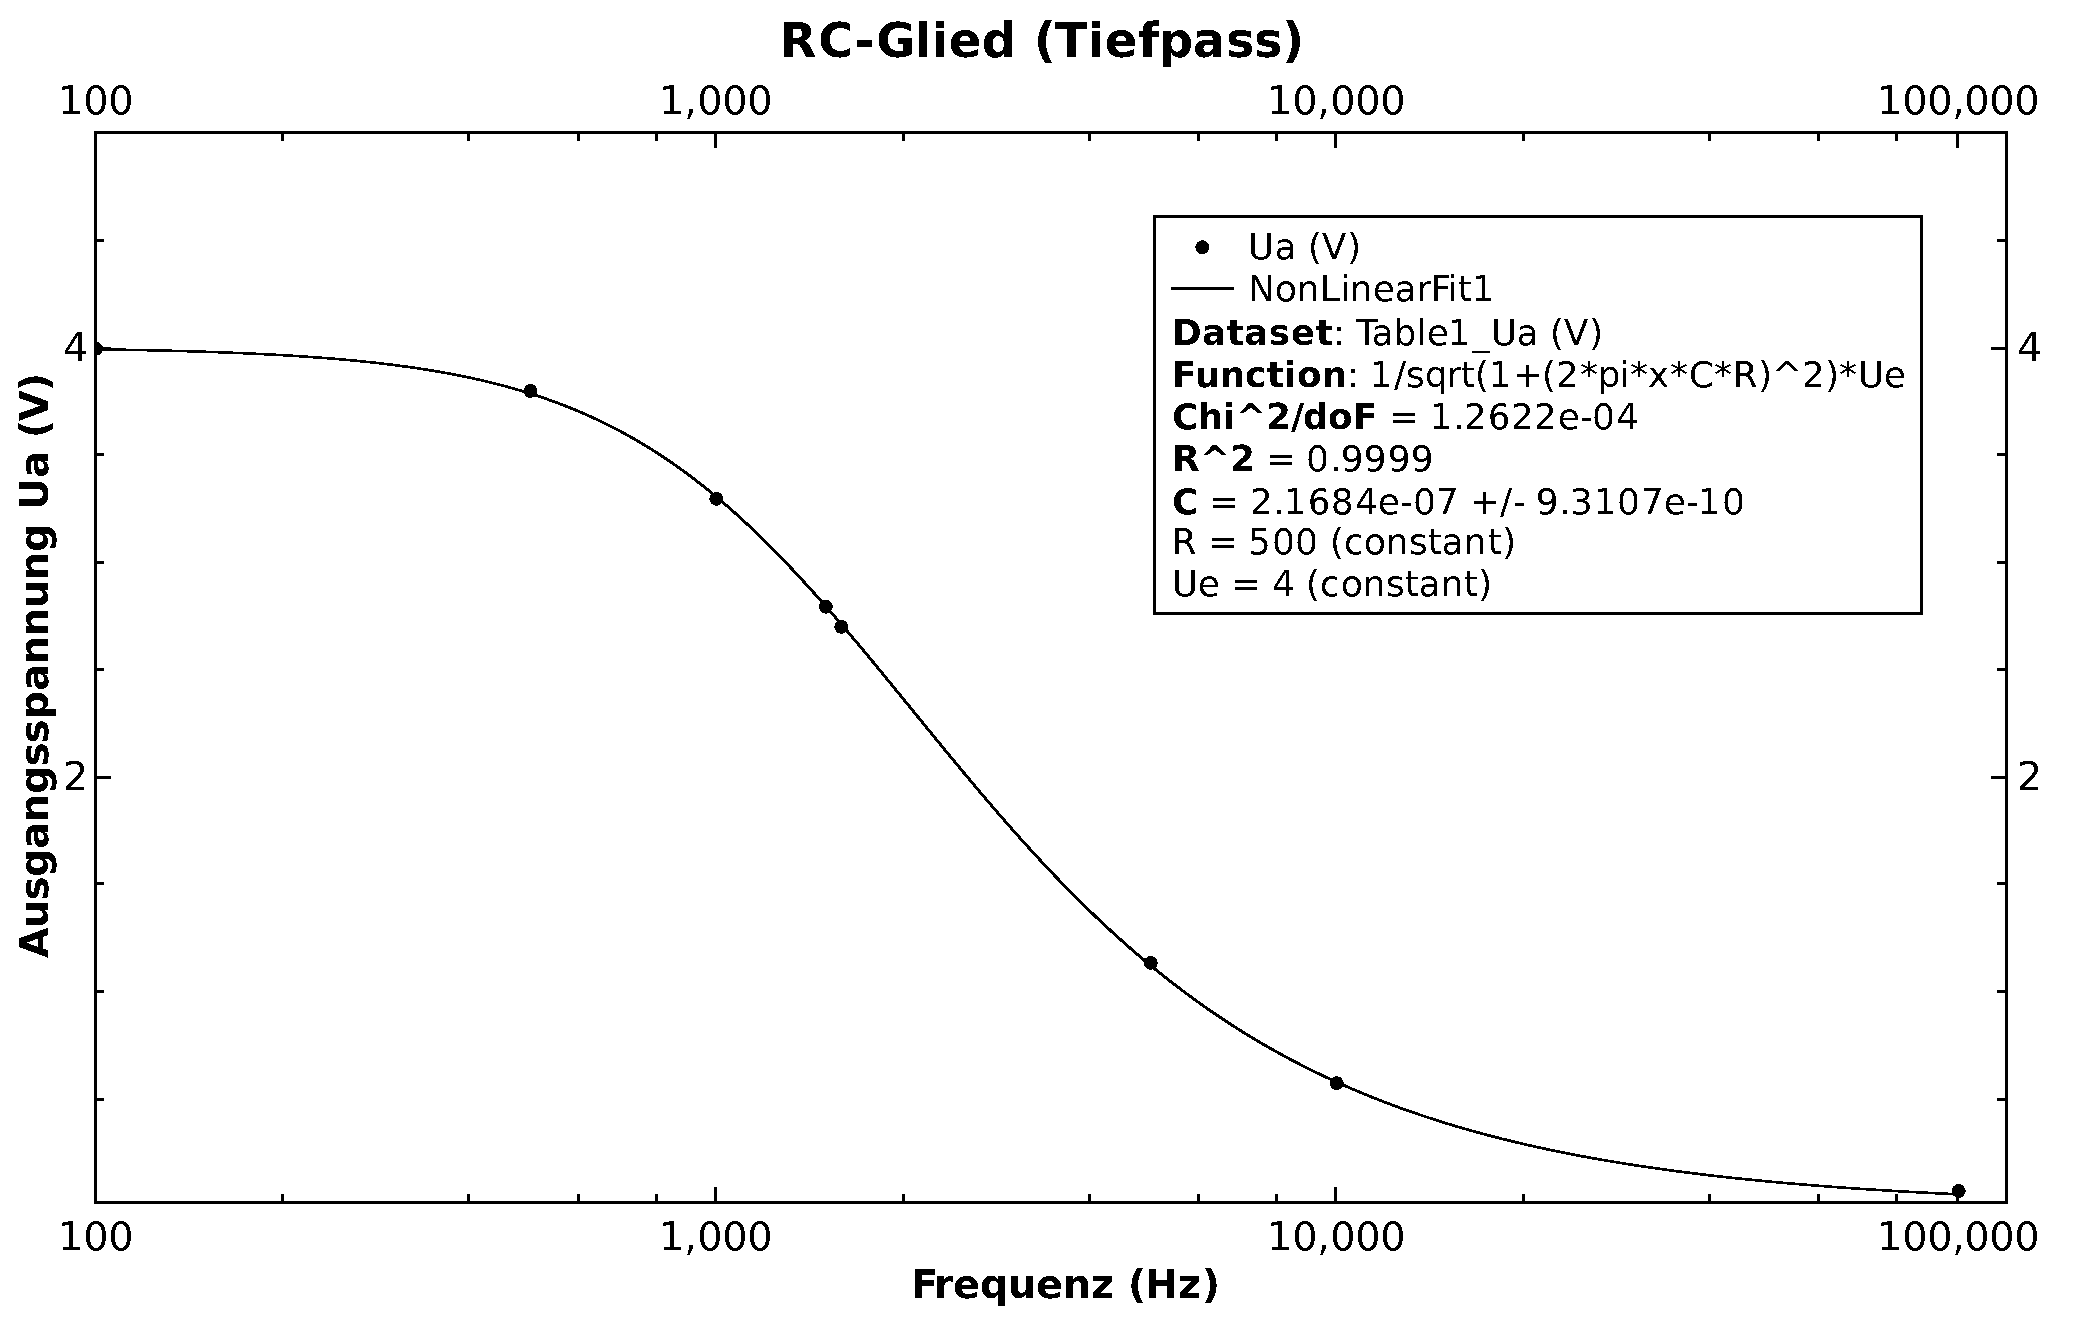
\includegraphics[width=.8\textwidth]{images/aufgabe5-betrag.pdf}
    \caption{Ausgangsspannung in Abh\"angigkeit der Frequenz}
    \label{fig:rcglied:spannung}
\end{figure}

Der aus diesem Fit erhaltene Wert f\"ur die Kapazit\"at betr\"agt:
\begin{equation*}
    C = \SI[separate-uncertainty = true]{0.21684 \pm 0.00093107}{\micro\farad}
\end{equation*}

Gerundet:
\begin{equation*}
    C = \SI[separate-uncertainty = true]{216.8 \pm 0.9}{\nano\farad}
\end{equation*}

\begin{figure}[th!]
    \centering
    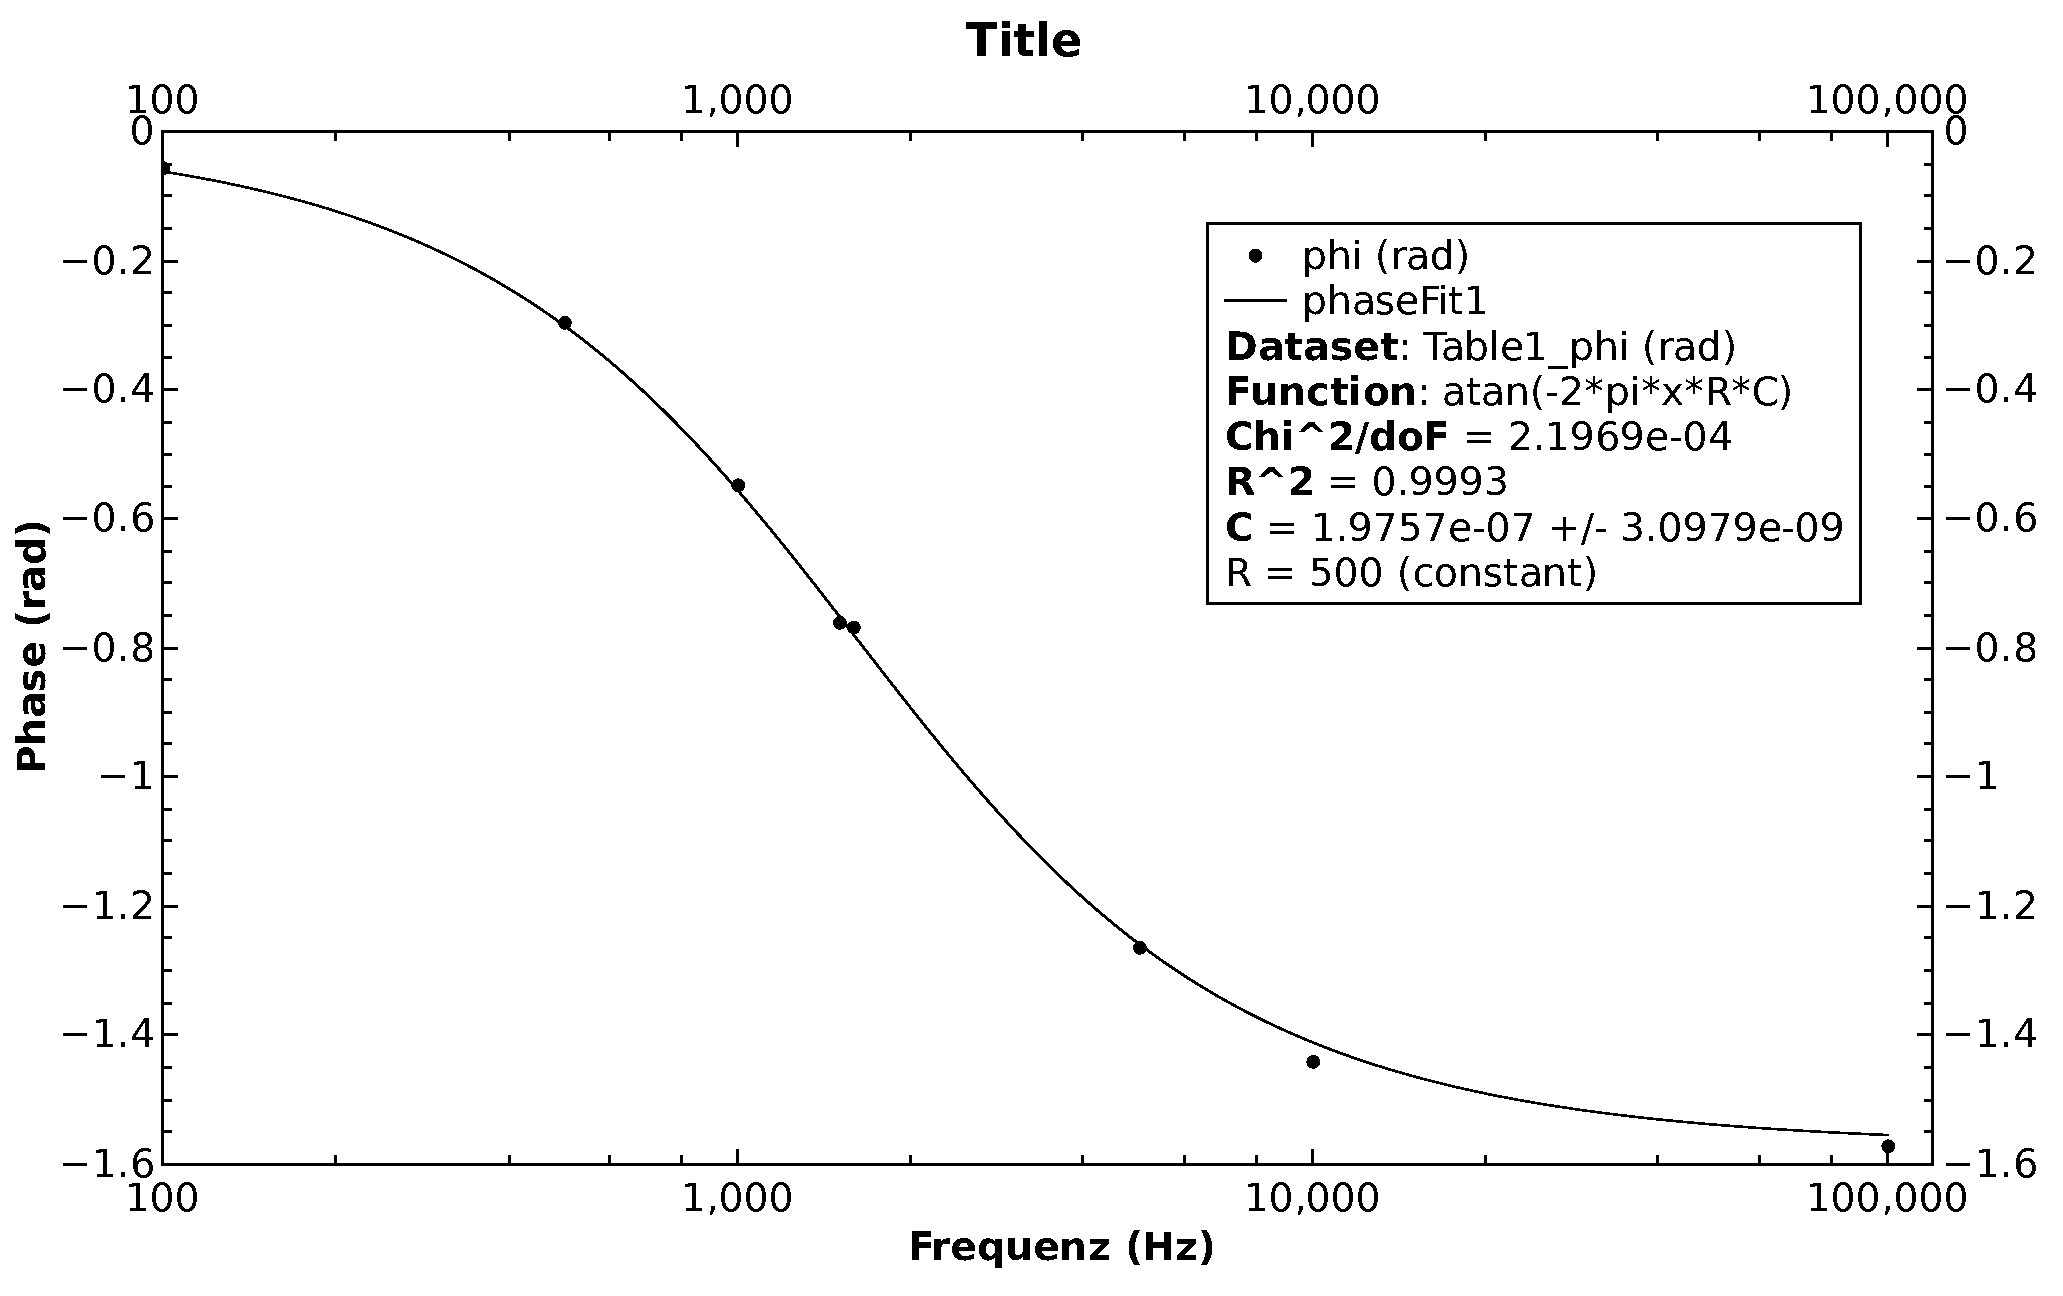
\includegraphics[width=.8\textwidth]{images/aufgabe5-phase.pdf}
    \caption{Phase $\varphi$ zwischen Ausgans- und Eingangsspannung in Abh\"angigkeit der Frequenz}
    \label{fig:rcglied:phase}
\end{figure}

In diesem Fit wurde die Kapazit\"at errechnet auf:
\begin{equation*}
    C = \SI[separate-uncertainty = true]{0.19757 \pm 0.0030979}{\micro\farad}
\end{equation*}

Gerundet:
\begin{equation*}
    C = \SI[separate-uncertainty = true]{198 \pm 3}{\nano\farad}
\end{equation*}

Mehr zu diesen Werten siehe im Abschnitt zur Diskussion der Ergebnisse.
